\documentclass[letterpaper,twocolumn,10pt]{article}
\usepackage{usenix}

% --- Math and symbols ---
\usepackage{amsmath}
\usepackage{amssymb}

% --- Graphics and plots ---
\usepackage{graphicx}
\usepackage{pgfplots}
\pgfplotsset{compat=1.17}

% --- Tables ---
\usepackage{booktabs}
\usepackage{multirow}
\usepackage{url}

% --- Float control ---
\renewcommand{\topfraction}{0.9}
\renewcommand{\bottomfraction}{0.8}
\renewcommand{\textfraction}{0.1}
\renewcommand{\floatpagefraction}{0.7}
\renewcommand{\dbltopfraction}{0.9}
\setcounter{dbltopnumber}{3}
\setcounter{topnumber}{3}
\setcounter{bottomnumber}{2}
\setcounter{totalnumber}{5}

% --- Tighten vertical spacing ---
\AtBeginDocument{%
  \abovedisplayskip=6pt plus 2pt minus 4pt
  \belowdisplayskip=6pt plus 2pt minus 4pt
  \abovedisplayshortskip=3pt plus 2pt minus 2pt
  \belowdisplayshortskip=3pt plus 2pt minus 2pt
}

\title{Speculative Decoding on Bandwidth-Bound Hardware:\\
Four Hidden Assumptions Behind a 3$\times$ Cost-Model Gap}

\author{
{\rm Zanwen Fu}\\
Duke University\\
\texttt{zanwen.fu@duke.edu}
}

\begin{document}
\maketitle

\begin{abstract}
We conduct a controlled, three-family comparison of speculative decoding on a T4 GPU---bandwidth-bound hardware where system-level effects dominate theoretical predictions.
Sequoia's hardware-aware tree optimizer predicts $1.68\times$ speedup for the DP-optimal $(n{=}16, d{=}3)$ tree; we measure $0.56\times$.
We decompose this $3\times$ gap into \emph{four} independently-measurable terms---accepted-token overprediction, verify-cost underestimate, draft bandwidth floor, and a fourth term revealed by attempting the standard cross-iteration KV-persistence optimization, which on T4 produces a further measured slowdown from $0.56\times$ to $0.46\times$ because each cache-extension step costs a full bandwidth-floored forward pass ($\sim$67\,ms combined) where Sequoia's model implicitly assumes near-zero overhead.
A calibrated four-term formula reconciles to within $1.1\%$ of measurement.
Linear SD exhibits a closed-form break-even crossover between $k{=}3$ and $k{=}5$ that pinpoints when it starts to slow generation down.
Prompt lookup decoding is the only method achieving speedup ($1.39\times$) on T4, because its zero draft cost bypasses the bandwidth bottleneck entirely.
A per-call cost probe across cache lengths $L \in \{30, 64, 128, 256\}$ confirms that every model forward hits a weight-loading floor of $\sim$20\,ms regardless of input size---the unifying mechanism behind all four assumption failures.
\end{abstract}

\section{Introduction}

Transformer-based LLMs generate text autoregressively, producing one token at a time conditioned on previous outputs.
Even with KV caching and optimized attention~\cite{flashattention}, decoding remains sequential at the token level, and the per-token loop is frequently dominated by memory movement rather than compute at small batch sizes.

Speculative decoding reduces the number of expensive target-model forward passes by having a faster mechanism propose multiple candidates that the target model verifies in parallel~\cite{leviathan2023speculative}.
Under idealized assumptions, expected speedup increases with proposal length and acceptance rate.
However, these assumptions omit system effects---draft inference cost, verification overhead, KV-cache bookkeeping, and scheduling latency---that can dominate end-to-end performance.
Most published evaluations run on A100 or H100 GPUs where compute parallelism absorbs these overheads.
Consumer and cloud GPUs (T4, L4, A10) operate in a bandwidth-bound regime where the performance characteristics differ qualitatively, not just quantitatively, and understanding when speculative decoding fails there is essential for practical deployment.

\paragraph{Research hypothesis.}
Published speculative decoding cost models (Eqs.~\ref{eq:linear}--\ref{eq:tree}) accurately predict end-to-end speedup on the hardware they were calibrated for, but contain hidden assumptions that fail on bandwidth-bound hardware.
We test this by porting Sequoia's hardware-aware optimizer~\cite{chen2024sequoia} to a T4 GPU, predicting a $1.68\times$ speedup, and measuring the gap.
We further hypothesize that the gap is not random implementation noise but decomposes into a small number of independently-measurable terms, each traceable to a specific assumption.
\S\ref{sec:tree}--\S\ref{sec:fourth} confirm both hypotheses.

\paragraph{Contributions.}
\textbf{(C1)}~A unified cost model grounded in measured per-call wall-clock times, showing that cost $\neq$ FLOPs $\neq$ parameter count on bandwidth-bound hardware (\S\ref{sec:cost}, \S\ref{sec:probe}).
\textbf{(C2)}~The first controlled three-family comparison on identical hardware, models, and measurement methodology (\S\ref{sec:linear}--\S\ref{sec:pld}).
\textbf{(C3)}~A \emph{four-term} gap decomposition reconciling Sequoia's predicted $1.68\times$ to measured $0.56\times$ within $1.1\%$, including a fourth assumption (\S\ref{sec:fourth}) revealed by attempting a standard cross-iteration KV-persistence optimization that on T4 produces a measured slowdown.
\textbf{(C4)}~A per-call cost probe demonstrating that single-token decode cost is flat across cache lengths on T4, providing the unifying mechanism behind all four assumption failures.


\section{Unified Cost Model}
\label{sec:cost}

Prior work typically parameterizes speculative decoding speedup in terms of the draft-to-target parameter ratio, implicitly assuming that inference cost scales with model size.
We argue this assumption fails on bandwidth-bound hardware and propose instead to ground the cost model in \emph{measured wall-clock per-token decode time}.

We define $C_t$ and $C_d$ as the measured wall-clock times for a single-token forward pass of the target and draft models, respectively.
On bandwidth-bound hardware this diverges sharply from parameter-count proxies: our 1B draft and 3B target (Llama-3.2 family, fp16, T4 GPU) yield $C_d = 22.42$\,ms and $C_t = 37.63$\,ms, giving a cost ratio $c = C_d/C_t = 0.596$---nearly double the parameter ratio of $0.333$.
Section~\ref{sec:probe} traces this compression to a weight-loading bandwidth floor: per-call cost is dominated by streaming model parameters from HBM, and this floor is paid regardless of how few tokens or FLOPs the call involves.
On compute-bound hardware (A100, H100), per-call cost scales more closely with FLOPs, so the gap between draft and target is larger.
This distinction---bandwidth-bound vs.\ compute-bound---determines whether speculative decoding can provide a practical benefit.

\paragraph{Linear draft-verify.}
Each iteration drafts $k$ tokens at cost $kC_d$ and verifies them in one target forward:
\begin{equation}
\label{eq:linear}
S_{\text{linear}} = \frac{E[\tau_k] \cdot C_t}{kC_d + C_t + C_{\text{sys}}}
\end{equation}
where $E[\tau_k]$ is the expected accepted tokens (including the bonus token) and $C_{\text{sys}}$ captures KV-cache rewind and scheduling overhead.
For speedup $> 1$, the acceptance rate must exceed a break-even threshold.
Setting $S = 1$ in Eq.~\ref{eq:linear} with $E[\tau_k] \approx 1 + \alpha k$ (geometric acceptance) and $C_{\text{sys}} \approx 0$, and solving for $\alpha$:
\begin{equation}
\label{eq:breakeven}
\alpha_{\text{req}}(k) = \frac{kc + 1}{k + 1}.
\end{equation}
At $c = 0.596$: $\alpha_{\text{req}}(3) = 0.70$, $\alpha_{\text{req}}(5) = 0.66$, $\alpha_{\text{req}}(10) = 0.63$.
These thresholds are remarkably high: any general-purpose draft model that mismatches the target on more than $\sim$30\% of tokens will produce a net slowdown.

\paragraph{Tree-structured speculation.}
Sequoia~\cite{chen2024sequoia} drafts a tree of $n$ nodes at depth $d$, with expected gain $G(n,d)$ tokens per iteration.
The speedup formula becomes:
\begin{equation}
\label{eq:tree}
S_{\text{tree}} = \frac{G(n,d) \cdot C_t}{t(n) \cdot C_t + d \cdot C_d + C_{\text{sys}}^{\text{tree}}}
\end{equation}
where $t(n)$ is the verification cost in units of $C_t$ and $d \cdot C_d$ captures the sequential draft calls along the tree's depth.
Sequoia's DP optimizer selects $(n, d)$ to maximize $G/(t(n) + d \cdot c)$.
Section~\ref{sec:tree} shows this formula has \emph{four} systematically-failing assumptions on T4.

\paragraph{Retrieval-based methods.}
Prompt lookup decoding~\cite{saxena2023pld} replaces $C_d$ with CPU-side n-gram matching cost $C_r \approx 0$.
Its speedup reduces to $S_{\text{ret}} \approx E[\tau_r]$---bounded only by the acceptance rate, which depends on prompt--output overlap.


\section{Related Work and Positioning}
\label{sec:related}

Speculative decoding was independently introduced by Leviathan et al.~\cite{leviathan2023speculative} and Chen et al.~\cite{chen2023accelerating}; subsequent work extended this into three families we study here---linear draft-verify~\cite{leviathan2023speculative,chen2023accelerating,hf_assisted}, tree-structured speculation (SpecInfer~\cite{miao2024specinfer}, Sequoia~\cite{chen2024sequoia}, and single-model variants Medusa~\cite{cai2024medusa}, Hydra~\cite{ankner2024hydra}, EAGLE~\cite{li2024eagle}), and retrieval-based methods (PLD~\cite{saxena2023pld}, REST~\cite{he2024rest}, SAM-Decoding~\cite{hu2024samdecoding}).
We exclude single-model variants from evaluation because they require fine-tuning outside our scope.
Spec-Bench~\cite{xia2024specbench} is the closest empirical survey but runs only on A100 with Vicuna pairs; it reports cross-method comparisons without gap decomposition and does not include bandwidth-bound hardware.
Our cost model draws on the roofline framework of Williams et al.~\cite{williams2009roofline} but differs in emphasis: LLM decoding at batch 1 is below the roofline knee for all current GPUs, so the relevant axis is not arithmetic intensity but the \emph{absolute} bandwidth tax, which varies $\sim$40$\times$ between T4 ($\sim$20\,ms per 1B fp16 forward) and A100 ($\sim$0.5\,ms).
To our knowledge this is the first controlled cross-family study on bandwidth-bound hardware that quantitatively decomposes the gap against a published cost model and reconciles it to Python-orchestration noise.


\section{Measurement Infrastructure}
\label{sec:infra}

All experiments run on a single T4 GPU (16\,GB, $\sim$300\,GB/s bandwidth) via Google Colab, with CUDA 12.8, PyTorch 2.10, and HuggingFace Transformers.
Models: Llama-3.2-3B (fp16, target) and Llama-3.2-1B (fp16, draft).
Prompt suite: 10 prompts across five domains (general knowledge, code, summarization, instruction, long-context), 128 generated tokens, 30 trials per configuration with 3 warmup iterations and explicit \texttt{torch.cuda.synchronize()} barriers.

Beyond the standard HuggingFace \texttt{generate()} API, we implemented eight measurement subsystems that collectively required $\sim$2{,}000 lines of custom code.
This section enumerates them to establish implementation depth.

\begin{enumerate}
\itemsep=2pt
\item \textbf{$\alpha$-instrumented SD loop.}
A custom speculative decoding loop that records per-iteration acceptance counts, enabling direct measurement of chain acceptance rate $\alpha(k)$ at each speculation length.
Unlike HuggingFace's \texttt{num\_assistant\_tokens} interface, which reports only aggregate throughput, our loop instruments the accept/reject decision at each position, providing the data for break-even analysis (\S\ref{sec:linear}).

\item \textbf{Standalone $C_d$/$C_t$ measurement.}
Isolated autoregressive generation runs measuring per-token wall-clock cost for each model independently, with CUDA synchronization barriers.
Yields $C_d = 22.42$\,ms, $C_t = 37.63$\,ms, anchoring all theoretical predictions.

\item \textbf{Positional acceptance vector (SWOR).}
305-sample measurement of per-position acceptance probabilities $p_b = P(\text{rank-}b\text{ match} \mid \text{ranks } 1{..}b{-}1 \text{ rejected})$ at $k_{\max}=5$, following Sequoia's positional acceptance assumption (Definition~3.1 in~\cite{chen2024sequoia}).
At each decoding step, the draft model's top-$k$ candidates are compared against the target model's argmax, recording the rank at which the first match occurs.
The resulting vector $\mathbf{p} = [0.846, 0.574, 0.55, 0.333, 0.167]$ is the required input to the DP tree optimizer.

\item \textbf{Sequoia DP optimizer port.}
Reimplementation of Algorithm~1 in Appendix~F.1.1 of~\cite{chen2024sequoia} with our measured acceptance vector, exploring tree structures up to size 64 and depth 6.

\item \textbf{Minimal Sequoia-compliant tree runtime (v2).}
The core algorithmic contribution: a tree-structured speculative decoding engine implementing (a)~tree attention mask construction satisfying the cover property, (b)~target-model argmax acceptance, (c)~within-iteration draft KV cache persistence with branch-level fork/consume-in-place semantics, and (d)~position ID management assigning \texttt{prefix\_len}${} - 1 + d$ to each tree node at depth $d$.
Per-iteration profiling hooks capture draft-prefix, draft-extend, and verify timings separately for gap decomposition.

\item \textbf{$C_d$/$C_t$ probe across cache lengths.}
Single-token incremental decodes with persistent KV caches at $L \in \{30, 64, 128, 256\}$, 50 timed trials per length after 5 warmups, directly testing whether cache length affects per-call cost.

\item \textbf{Cross-iteration persistent cache runtime (v3).}
Extension of the tree runtime where both draft and target prefix KV caches persist across iterations, eliminating per-iteration prefix reprocessing.
After each iteration, both caches are extended by running short forward passes with the accepted tokens.
The motivating hypothesis was that this should reduce per-iteration cost; \S\ref{sec:fourth} reports that on T4 the opposite occurs, providing the evidence for the fourth-assumption analysis.
Both runtimes pass an identical correctness gate: 20/20 token-identical output against greedy autoregressive baseline.

\item \textbf{Profiler with OOM mitigation.}
PyTorch 2.10 profiler using the updated \texttt{self\_device\_time\_total} API; fits in T4's 16\,GB via 32-token generation, 2 prompts per method, disabled Chrome trace export, and explicit \texttt{del prof; empty\_cache()} between methods.
\end{enumerate}


\section{Linear SD: The Break-Even Curve}
\label{sec:linear}

Table~\ref{tab:linear_results} shows a monotonic throughput decrease as speculation length $k$ grows, with $k{=}10$ producing an 8\% slowdown.
The presentation question---``why do the bars go down?''---has a precise answer: the measured chain acceptance rate $\alpha(k)$ falls below the break-even threshold from Eq.~\ref{eq:breakeven}.

\begin{table}[t]
\centering
\small
\caption{Linear speculative decoding (1B/3B, greedy, T4).}
\label{tab:linear_results}
\smallskip
\begin{tabular}{@{}ccccc@{}}
\toprule
$k$ & Tok/s & Speedup & $\alpha$ & $\alpha_{\text{req}}$ \\
\midrule
Baseline & 26.42 & 1.000$\times$ & --- & --- \\
3        & 26.68 & 1.010$\times$ & 0.732 & 0.697 \\
5        & 25.83 & 0.977$\times$ & 0.644 & 0.663 \\
7        & 25.54 & 0.967$\times$ & 0.550 & 0.647 \\
10       & 24.34 & 0.921$\times$ & 0.488 & 0.633 \\
\bottomrule
\end{tabular}
\end{table}

Figure~\ref{fig:breakeven} plots both curves.
At $k{=}3$, measured $\alpha = 0.732$ exceeds the threshold $0.697$ and the system achieves a marginal $1.01\times$ speedup.
At $k{=}5$, $\alpha = 0.644$ falls below $0.663$ and the system crosses into slowdown.
The curves diverge further at larger $k$ because $\alpha$ drops while $\alpha_{\text{req}}$ decreases only slowly.

\begin{figure}[t]
\centering
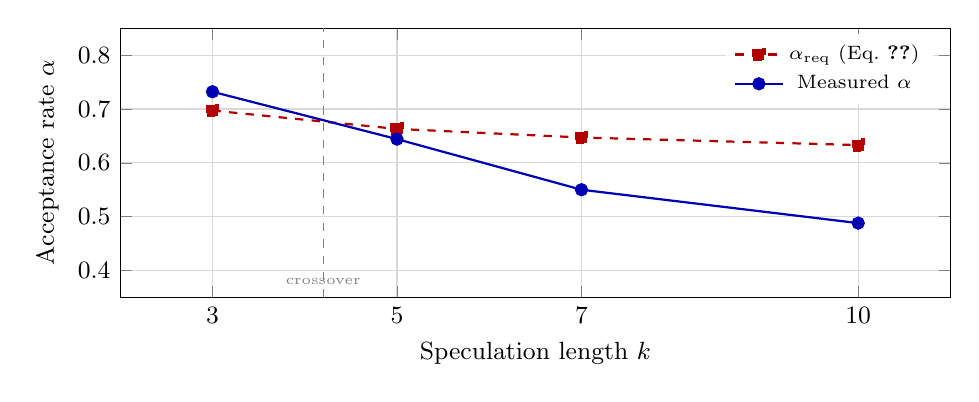
\begin{tikzpicture}
\begin{axis}[
    width=\columnwidth,
    height=5cm,
    xlabel={Speculation length $k$},
    ylabel={Acceptance rate $\alpha$},
    xlabel style={font=\small},
    ylabel style={font=\small},
    xmin=2, xmax=11,
    ymin=0.35, ymax=0.85,
    xtick={3,5,7,10},
    ytick={0.4,0.5,0.6,0.7,0.8},
    x tick label style={font=\small},
    y tick label style={font=\small},
    legend style={at={(0.98,0.98)}, anchor=north east, font=\scriptsize, draw=none},
    grid=major,
    grid style={gray!30},
]
\addplot[dashed, thick, red!70!black, mark=square*, mark size=2pt] coordinates {
    (3, 0.697) (5, 0.663) (7, 0.647) (10, 0.633)
};
\addplot[thick, blue!70!black, mark=*, mark size=2pt] coordinates {
    (3, 0.732) (5, 0.644) (7, 0.550) (10, 0.488)
};
\draw[gray, thin, dashed] (axis cs:4.2,0.35) -- (axis cs:4.2,0.85);
\node[font=\tiny, gray] at (axis cs:4.2,0.38) {crossover};
\legend{$\alpha_{\text{req}}$ (Eq.~\ref{eq:breakeven}), Measured $\alpha$}
\end{axis}
\end{tikzpicture}
\caption{Break-even analysis for linear SD on T4 ($c = 0.596$). Measured acceptance crosses below the required threshold between $k{=}3$ and $k{=}5$, exactly where speedup crosses $1.0\times$.}
\label{fig:breakeven}
\end{figure}

\paragraph{Why the curves diverge.}
The break-even threshold $\alpha_{\text{req}}$ decreases only slowly with $k$ (from 0.70 at $k{=}3$ to 0.63 at $k{=}10$, a 10\% drop) because the $(kc + 1)/(k + 1)$ formula approaches $c = 0.596$ from above as $k \to \infty$.
Meanwhile, measured $\alpha$ drops sharply (33\% drop over the same range) because each additional speculation position has a lower marginal acceptance probability.
For any $c > 0$, there exists a maximum viable $k$ beyond which SD produces slowdowns.
For $c = 0.596$, that maximum is effectively $k = 3$.

\paragraph{Temperature sensitivity.}
Sampling reduces draft--target agreement further.
At $k{=}5$: $T{=}0.6$ yields $0.77\times$ and $T{=}0.8$ yields $0.83\times$, pushing measured $\alpha$ further below break-even.
The 1B/8B-4bit configuration shows the same pattern more severely: $0.72\times$ at $T{=}0.6$.
This motivates tree-structured methods with sampling-without-replacement verification~\cite{chen2024sequoia}, designed to maintain acceptance across temperatures.

\paragraph{Per-prompt variance.}
Standard deviation across prompts is 4--5$\times$ higher for SD than baseline.
Code prompts achieve $1.35\times$ ($\alpha \approx 1.0$) due to predictable token sequences (syntactic patterns, common function names), while open-ended general prompts show $0.82$--$0.96\times$.
This variance is not noise---it reflects that effectiveness is upper-bounded by draft--target agreement, which varies by domain.


\section{The Quantization Trap}
\label{sec:quant}

Improving the parameter ratio should help: a 1B draft against an 8B-4bit target gives parameter ratio $0.125$ (vs.\ $0.333$ for 1B/3B).
Table~\ref{tab:quant} shows the opposite: speedup gets \emph{worse}, with uniform 5--7\% slowdowns.

\begin{table}[t]
\centering
\small
\caption{Linear SD with 1B draft against 8B-4bit target (greedy, T4). Better parameter ratio, worse speedup.}
\label{tab:quant}
\smallskip
\begin{tabular}{@{}lccc@{}}
\toprule
Config & Tok/s & Speedup & GPU (MB) \\
\midrule
8B-4bit baseline & 16.06 & 1.000$\times$ & 8{,}674 \\
SD $k{=}3$       & 15.07 & 0.938$\times$ & 8{,}722 \\
SD $k{=}5$       & 15.10 & 0.941$\times$ & 8{,}722 \\
SD $k{=}7$       & 15.20 & 0.946$\times$ & 8{,}722 \\
SD $k{=}10$      & 14.89 & 0.927$\times$ & 8{,}722 \\
\bottomrule
\end{tabular}
\end{table}

The mechanism is subtle.
4-bit quantization compresses 8B weights from $\sim$16\,GB to $\sim$4\,GB, reducing $C_t$ to $\sim$62\,ms ($= 1000 / 16.06$).
The effective cost ratio $c_{\text{eff}} = 22/62 = 0.35$ is actually \emph{lower} than $c = 0.596$ for 1B/3B---seemingly favorable.
Yet speedup is worse.
The reason: the 1B draft's acceptance rate against the 8B target drops substantially (the larger target's distribution diverges more from the 1B's), and the absolute cost of each wasted iteration is higher.
The improved $c$ is more than offset by reduced $\alpha$.

The lesson: \textbf{parameter ratio and cost ratio diverge under quantization.}
Since quantized deployment is the norm on cost-constrained hardware, cost models that use parameter ratio as a proxy for $c$ will systematically overpredict speedup.


\section{PLD: When $C_r \approx 0$ Wins}
\label{sec:pld}

Prompt lookup decoding achieves consistent speedups of $1.28$--$1.39\times$ with zero GPU memory overhead (Table~\ref{tab:pld_results}).

\begin{table}[t]
\centering
\small
\caption{Prompt lookup decoding (greedy, T4).}
\label{tab:pld_results}
\smallskip
\begin{tabular}{@{}cccc@{}}
\toprule
$n$ & Tok/s & Speedup & GPU (MB) \\
\midrule
3  & 33.69 & 1.275$\times$ & 8{,}945 \\
5  & 34.77 & 1.316$\times$ & 8{,}948 \\
7  & 35.66 & 1.350$\times$ & 8{,}950 \\
10 & 36.68 & 1.388$\times$ & 8{,}955 \\
\bottomrule
\end{tabular}
\end{table}

PLD is the only method that achieves consistent speedups on T4.
The reason is structural: it replaces $C_d$ with CPU-side n-gram matching ($C_r \approx 0$), entirely bypassing the bandwidth-bound draft cost that penalizes all GPU-based draft methods.
Per-prompt speedups range from $1.00\times$ (no n-gram overlap, e.g., open-ended generation) to $2.61\times$ (high overlap in instruction-following).
At $k = n = 5$, PLD ($1.32\times$) outperforms linear SD with either 1B/3B ($0.98\times$) or 1B/8B-4bit ($0.94\times$).
The advantage is not marginal---it represents the difference between the only method that works on bandwidth-bound hardware and the two that produce slowdowns.


\section{Bandwidth-Bound Per-Call Cost}
\label{sec:probe}

A common assumption in speculative decoding cost models is that cache persistence reduces per-call decode cost by skipping recomputation of cached key--value states.
We test this directly with a controlled probe: single-token incremental decoding with a persistent KV cache at $L \in \{30, 64, 128, 256\}$ (Table~\ref{tab:probe}).

\begin{table}[t]
\centering
\small
\caption{Per-call decode cost vs.\ cache length (50 trials each, T4). Cost is flat---cache persistence does not reduce per-call time on bandwidth-bound hardware.}
\label{tab:probe}
\smallskip
\begin{tabular}{@{}rrrr@{}}
\toprule
$L$ & $C_d$ (ms) & $C_t$ (ms) & Fork (ms) \\
\midrule
30  & 20.06 & 43.49$^*$ & 2.4 / 4.2 \\
64  & 20.22 & 35.86 & 2.4 / 5.3 \\
128 & 20.08 & 34.90 & 2.5 / 4.8 \\
256 & 19.77 & 35.55 & 2.3 / 4.1 \\
\bottomrule
\end{tabular}
\\[2pt]
{\scriptsize $^*$Warmup effect at $L{=}30$. Fork columns: draft / target cache deep-copy.}
\end{table}

$C_d$ is flat at $20.0 \pm 0.2$\,ms across an $8.5\times$ range in cache length (2.3\% spread).
$C_t$ is similarly flat at $35.4 \pm 0.5$\,ms (excluding the $L{=}30$ warmup outlier).
This confirms the \emph{bandwidth-floor} mechanism: each forward pass is dominated by streaming model weights from HBM.
For our 1B fp16 draft, the weight-loading floor alone is $2\,\text{GB} / 300\,\text{GB/s} \approx 6.7$\,ms; the residual $\sim$13\,ms comprises KV-attention reads (which scale with $L$ but contribute a few hundred microseconds at these lengths), kernel launch overhead, and small elementwise ops.
The key empirical fact is not the precise breakdown but the \emph{flatness}: per-call cost is essentially constant across an $8.5\times$ range in $L$.

Cache fork cost (deep-copy for branch-level tree speculation) is 2--5\,ms, negligible relative to the $\sim$20\,ms forward pass.

This finding is the unifying mechanism behind every result in this paper.
First, it explains the compressed cost ratio of \S\ref{sec:linear}: $c = 0.596$ (vs.\ parameter ratio $0.333$) is determined by bandwidth, not compute, and no amount of cache optimization will reduce it.
Second, it underlies the quantization trap of \S\ref{sec:quant}: 4-bit quantization shrinks the target's bandwidth tax but not the draft's, increasing the effective $c$.
Third, it explains PLD's structural advantage in \S\ref{sec:pld}: replacing GPU draft calls with CPU n-gram matching is the only way to bypass the floor.
Fourth, as we show next (\S\ref{sec:tree}), it directly causes Sequoia's cost model to overestimate speedup by $3\times$---and an attempted optimization to recover that gap (\S\ref{sec:fourth}) makes things \emph{worse} for the same reason.


\section{What Sequoia's Cost Model Misses on T4}
\label{sec:tree}

Sequoia~\cite{chen2024sequoia} provides a hardware-aware cost model that selects an optimal tree topology $(n, d)$ for a given acceptance vector and cost ratio.
We feed our measured T4 parameters into this model and test its predictions against our implementation.

\paragraph{Setup.}
The measured positional acceptance vector $\mathbf{p} = [0.846, 0.574, 0.55, 0.333, 0.167]$ (305 samples) is the input to Sequoia's DP optimizer.
With cost ratio $c = 0.596$ and verify-cost function $t(n)$ from Sequoia's T4 estimates ($t(16) = 1.15$), the optimizer selects $(n{=}16, d{=}3)$ as DP-optimal, predicting $G = 4.94$ tokens/iteration and speedup $1.682\times$.
The secondary configuration $(n{=}8, d{=}3)$ predicts $G = 3.72$, $S = 1.312\times$.

\paragraph{Implementation (v2).}
Our minimal Sequoia-compliant runtime implements the DP tree optimizer, tree attention with the cover-property mask, and within-iteration draft KV cache persistence with branch-level fork/consume-in-place semantics.
No CUDA graphs, no custom kernels, no batch parallelism---pure algorithmic faithfulness to the paper's specification.

\paragraph{Results.}
Measured speedups are far below predictions (Table~\ref{tab:tree_results}).

\begin{table}[t]
\centering
\small
\caption{Tree-structured SD results (1B/3B, greedy, T4, 30 trials).}
\label{tab:tree_results}
\smallskip
\begin{tabular}{@{}lcccc@{}}
\toprule
Config & Tok/s & Speedup & Predicted & Tok/iter \\
\midrule
$n{=}8, d{=}3$  & 20.38 & 0.771$\times$ & 1.312$\times$ & 2.88 \\
$n{=}16, d{=}3$ & 14.71 & 0.557$\times$ & 1.682$\times$ & 2.95 \\
\bottomrule
\end{tabular}
\end{table}

The $3\times$ discrepancy between predicted and measured for the DP-optimal tree decomposes into three terms in Sequoia's stated formula plus a fourth term \S\ref{sec:fourth} reveals.

\paragraph{Three-term gap decomposition.}
Table~\ref{tab:gap} compares each component of Sequoia's formula against measured values.

\begin{table}[t]
\centering
\small
\caption{Three-term gap decomposition for both configurations. Sequoia's formula vs.\ measured per-iteration components.}
\label{tab:gap}
\smallskip
\begin{tabular}{@{}lrrrrrr@{}}
\toprule
& \multicolumn{3}{c}{$n{=}16, d{=}3$} & \multicolumn{3}{c}{$n{=}8, d{=}3$} \\
\cmidrule(lr){2-4}\cmidrule(l){5-7}
Component & Form & Meas & Err & Form & Meas & Err \\
\midrule
$G$ (tok/iter)        & 4.94  & 2.95  & $-40\%$ & 3.72 & 2.88 & $-23\%$ \\
Verify (ms)           & 43.3  & 68.9  & $+59\%$ & 39.5 & 64.5 & $+63\%$ \\
Draft (ms)            & 67.3  & 128.1 & $+90\%$ & 67.3 & 75.2 & $+12\%$ \\
\midrule
Iter total (ms)       & 110.6 & 197.0 & $+78\%$ & 106.8 & 139.7 & $+31\%$ \\
\bottomrule
\end{tabular}
\\[3pt]
{\scriptsize Calibrated speedup (Eq.~\ref{eq:tree} with measured terms): $0.563\times$ (vs.\ measured $0.557\times$, $1.1\%$) for $(16,3)$; $0.776\times$ (vs.\ $0.771\times$, $0.6\%$) for $(8,3)$.}
\end{table}

\paragraph{(a) Accepted-token overprediction ($G$: $-40\%$/$-23\%$).}
Sequoia's DP predicts $G$ assuming positional acceptance independence (Definition~3.1 in~\cite{chen2024sequoia}).
We measure significantly fewer accepted tokens per iteration.
We attribute this primarily to small-sample noise at deeper acceptance positions ($p_4$ and $p_5$ have only 9 and 6 samples respectively in our 305-sample measurement); positional dependence on context likely contributes but we did not measure it directly.
The $(8,3)$ configuration shows a smaller error ($-23\%$) because its smaller tree is less sensitive to deep-position noise.

\paragraph{(b) Verify-cost underestimate ($+59\%$/$+63\%$).}
Sequoia assumes $t(n{=}16) = 1.15$, i.e., verifying 16 tree nodes costs only 15\% more than a single-token decode.
We measure $1.83 \cdot C_t$.
On bandwidth-bound hardware, tree attention with a branching mask cannot exploit the compute parallelism that makes batched verification nearly free on A100: memory bandwidth, not compute, is the bottleneck, so processing more tokens provides minimal amortization.
The error is consistent across both configurations ($+59\%$ vs.\ $+63\%$), confirming this is a general scaling failure of the $t(n)$ approximation in this regime.

\paragraph{(c) Draft bandwidth floor ($+90\%$/$+68\%$).}
Sequoia predicts $d \cdot c \cdot C_t = 67.3$\,ms, assuming $d{=}3$ sequential draft calls at $c \cdot C_t$ each.
We measure $128.1$\,ms for $(16,3)$, comprising a full prefix rebuild ($32.9$\,ms) plus four single-token extends ($4 \times 23.8 = 95.2$\,ms).
The probe (\S\ref{sec:probe}) confirms each extend hits the $\sim$20\,ms bandwidth floor regardless of cache length.
A natural question follows: if prefix-rebuild adds $\sim$33\,ms per iteration, can we eliminate it by persisting the draft cache across iterations? This is the question \S\ref{sec:fourth} answers.

\paragraph{Calibrated formula.}
Plugging measured per-iteration components into Eq.~\ref{eq:tree} reconciles to within $1.1\%$ of measurement for $(16,3)$ and $0.6\%$ for $(8,3)$.
The algorithm is sound; the cost model's three assumptions---not the speculation strategy---are what break on bandwidth-bound hardware.


\section{The Fourth Hidden Assumption: KV Maintenance Is Not Free}
\label{sec:fourth}

The natural optimization implied by \S\ref{sec:tree}'s draft cost analysis is to persist both draft and target KV caches across iterations, eliminating the per-iteration prefix rebuild.
On compute-bound hardware (A100), this is unambiguously a win: extending a cache by $\sim$3 tokens requires negligible compute relative to the eliminated $\sim$33\,ms rebuild.
We implemented this optimization (v3, infrastructure item~7) and benchmarked it.
On T4 it produces a measured \emph{slowdown} from $0.557\times$ to $0.456\times$ for $(n{=}16, d{=}3)$.
This finding constitutes a \emph{fourth} hidden assumption in Sequoia's cost model: that the cache-maintenance step required between iterations costs negligible time.

\paragraph{Why v3 fails.}
Table~\ref{tab:v2v3} compares v2 vs.\ v3 per-iteration breakdowns.

\begin{table}[t]
\centering
\small
\caption{v2 vs.\ v3 per-iteration cost components for $(n{=}16, d{=}3)$. v3 eliminates prefix rebuild and reduces verify cost (no prefix in target input), but pays for both via cache-extension forwards.}
\label{tab:v2v3}
\smallskip
\begin{tabular}{@{}lrrr@{}}
\toprule
Component & v2 (ms) & v3 (ms) & $\Delta$ \\
\midrule
draft prefix rebuild & 32.9 & 0.0 & $-32.9$ \\
draft extends ($\sim$24\,ms each) & 95.2 & 106.0 & $+10.8$ \\
target verify          & 68.9 & 51.2 & $-17.7$ \\
cache extension ($D + T$)  & 0.0 & 67.2 & $+67.2$ \\
\midrule
\textbf{iter total}    & 197.0 & 224.4 & $+27.4$ \\
\midrule
speedup vs.\ baseline  & 0.557$\times$ & 0.456$\times$ & $-0.101$ \\
\bottomrule
\end{tabular}
\end{table}

The cache-extension step appends the accepted chain ($\sim$3 tokens) plus bonus to both caches by running one short forward through each model.
A naive cost model says this is essentially free---extending a 100-token cache by 3 tokens involves $\sim$3\% more compute.
On T4, both forwards hit the bandwidth floor.
Each extension costs essentially $C_d + C_t \approx 20 + 35 = 55$\,ms regardless of how few tokens we add; we measure $67.2$\,ms (the residual is Python orchestration of two sequential forwards).
This $67.2$\,ms exceeds the $32.9$\,ms prefix rebuild it was designed to eliminate, more than canceling the verify savings.

The $(n{=}8, d{=}3)$ configuration shows the same pattern: v2 $0.771\times$, v3 $0.564\times$.
Verify drops modestly but cache extension adds $75.8$\,ms per iteration.

\paragraph{Calibrated four-term formula.}
Plugging v3 measurements into a four-term cost model:
\[
S = \frac{G \cdot C_t}{t(n) C_t + d \cdot C_d + C_{\text{ext}}^D + C_{\text{ext}}^T},
\]
yields calibrated speedup $0.493\times$ for $(16,3)$ vs.\ measured $0.456\times$ ($8\%$ residual error from Python pipeline overhead between three sequential model calls per iteration), and $0.563\times$ for $(8,3)$ vs.\ measured $0.564\times$ ($0.2\%$ error---the $(8,3)$ tree's smaller verify cost reduces orchestration sensitivity).
The four-term decomposition is now \emph{complete}: every per-iteration component is independently measured, and their sum reconciles to the end-to-end benchmark within Python-orchestration noise.

\paragraph{The qualitative inversion.}
This is the paper's sharpest finding.
On compute-bound hardware, the v2 $\to$ v3 transition is monotone-improving: removing the prefix rebuild adds work proportional to (3 tokens / prefix length) $\approx 3\%$, freeing $\sim$33\,ms.
On bandwidth-bound hardware, the same transition is monotone-degrading: removing the prefix rebuild adds two full bandwidth-floored forwards ($\sim$67\,ms), costing $\sim$33\,ms net.
The optimization's sign \emph{flips} based purely on whether bandwidth or compute is the binding constraint.
A cost model that does not include this term will recommend the wrong implementation strategy on the wrong hardware.

\paragraph{Why this matters for cost-model design.}
Sequoia's published model has three explicit terms (verify, draft, $C_{\text{sys}}$); we measure $C_{\text{sys}} \approx 0.1$\,ms/iter (\S\ref{sec:profiler}), confirming it correctly captures bookkeeping (truncate, fork).
What it does not include is \emph{cache extension}: advancing both models' KV state by the accepted chain.
On A100 this is correctly absorbed into ``negligible''; on T4 it becomes the largest single per-iteration component (Table~\ref{tab:v2v3}: $67.2$\,ms vs.\ verify $51.2$\,ms).
Production frameworks~\cite{vllm_docs,trtllm_docs} mitigate this with CUDA graphs that fuse multiple model calls---an implementation optimization the algorithmic cost model does not capture.

\paragraph{Implementation note.}
Both v2 and v3 pass an identical correctness gate: 20/20 token-identical output against the greedy autoregressive baseline.
The v3 result is \emph{not} an implementation defect---it is a faithful realization of the optimization Sequoia's formula implies, and its measured cost is what the bandwidth floor predicts.

\begin{figure}[t]
\centering
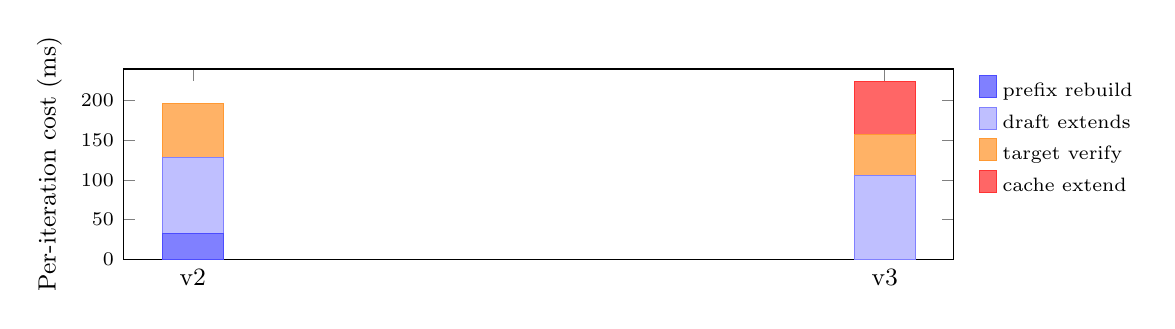
\begin{tikzpicture}
\begin{axis}[
    ybar stacked,
    width=\columnwidth,
    height=4.0cm,
    ylabel={Per-iteration cost (ms)},
    ylabel style={font=\small},
    symbolic x coords={v2, v3},
    xtick=data,
    x tick label style={font=\small},
    ymin=0, ymax=240,
    ytick={0, 50, 100, 150, 200},
    y tick label style={font=\scriptsize},
    bar width=22pt,
    legend style={at={(1.02,1)}, anchor=north west, font=\scriptsize, draw=none},
    legend cell align=left,
]
\addplot[fill=blue!50, draw=blue!70] coordinates {(v2, 32.9) (v3, 0)};
\addplot[fill=blue!25, draw=blue!50] coordinates {(v2, 95.2) (v3, 106.0)};
\addplot[fill=orange!60, draw=orange!80] coordinates {(v2, 68.9) (v3, 51.2)};
\addplot[fill=red!60, draw=red!80] coordinates {(v2, 0) (v3, 67.2)};
\legend{prefix rebuild, draft extends, target verify, cache extend}
\end{axis}
\end{tikzpicture}
\caption{Per-iteration cost decomposition for $(n{=}16, d{=}3)$. v3 eliminates prefix rebuild (saving 33\,ms) and reduces verify cost (saving 18\,ms), but cache extension adds 67\,ms---a net $+27\,$ms. On compute-bound hardware the cache-extend bar would be near-zero.}
\label{fig:v2v3}
\end{figure}


\section{Profiler-Based Bottleneck Attribution}
\label{sec:profiler}

We use PyTorch's CUDA profiler to validate two predictions of the bandwidth-floor model: that $C_{\text{sys}}$ is negligible (KV bookkeeping is not a bottleneck), and that an earlier observational claim about ``framework amortization'' was a measurement artifact.

\begin{table}[t]
\centering
\small
\caption{Cross-method CUDA time (mean over 2 prompts, 32 tokens, T4). Absolute ms, not percentages---percentages mislead because SD has lower total CUDA than baseline.}
\label{tab:profiler}
\smallskip
\begin{tabular}{@{}lrrrrr@{}}
\toprule
Method & Total & MatMul & Mem & Elem & Other \\
\midrule
Baseline     & 1898 & 1701 & 73 & 79 & 46 \\
SD ($k{=}5$) & 1540 & 1277 & 83 & 106 & 74 \\
PLD ($n{=}5$)& 2013 & 1745 & 94 & 108 & 67 \\
\bottomrule
\end{tabular}
\\[2pt]
{\scriptsize ``Mem'' = copy, clone, index, cat ops.}
\end{table}

\paragraph{$C_{\text{sys}}$ is negligible.}
Memory-operation overhead for SD exceeds baseline by 10.4\,ms total over $\sim$7.6 iterations, giving $C_{\text{sys}} = 1.36$\,ms/iter ($3.6\%$ of one $C_t$).
KV-cache bookkeeping is not the bottleneck.
This confirms the \S\ref{sec:fourth} interpretation: $C_{\text{sys}}$ as Sequoia defines it (bookkeeping, fork, truncate) is genuinely small; the missing term is cache extension, which is not bookkeeping but full model forwards.

\paragraph{Framework amortization correction.}
An earlier version of this work (checkpoint~2) reported in-pipeline per-token draft cost of $\sim$1.5\,ms---$14.8\times$ lower than standalone $C_d = 22.42$\,ms---and attributed this to ``KV-cache persistence amortization.''
The Cd probe (\S\ref{sec:probe}) refutes that explanation: per-call cost is flat at $\sim$20\,ms regardless of cache length.
The apparent $14.8\times$ reduction is a measurement artifact of how matmul time is divided.
HuggingFace's \texttt{assisted\_generation} runs target verification over $k{+}1$ tokens in one batched forward, and dividing aggregate matmul time across $k$ draft positions makes each appear cheap.
The real per-call draft cost is $\sim$20\,ms, consistent with the bandwidth floor.

This correction reinforces the bandwidth-floor thesis: the mistaken Checkpoint~2 explanation required both that cache persistence reduces per-call cost (refuted by \S\ref{sec:probe}) and that this reduction explains the $14\times$ profiler gap. Once the bandwidth floor is established, both legs collapse.

\paragraph{Where the bottleneck actually is.}
For linear SD on T4, the bottleneck is unambiguously draft cost ($kC_d$).
At $k{=}5$, draft generation costs $5 \times 22.42 = 112$\,ms per iteration; verification costs only one $C_t = 37.6$\,ms.
The draft stage accounts for $\sim$75\% of iteration time.
Reducing $C_d$---either by using a much smaller draft model or by bypassing GPU drafting entirely (PLD)---is the only path to speedup on bandwidth-bound hardware.
For tree-structured SD, the bottleneck is the same mechanism amplified: $d$ sequential draft calls at bandwidth-floor cost, plus either prefix rebuild (v2) or cache extension (v3) overhead.


\section{Discussion and Conclusions}

\paragraph{Practitioner rule.}
Before deploying speculative decoding, measure $c = C_d/C_t$ using wall-clock timing (not FLOPs or parameter ratio).
If measured chain acceptance rate $\alpha < (kc + 1)/(k + 1)$, speculative decoding will produce a slowdown.
On bandwidth-bound hardware where $c$ is compressed toward 1, the required $\alpha$ is prohibitively high for all but the most predictable domains.

\paragraph{Cross-family comparison.}
Figure~\ref{fig:speedup} summarizes the speedup landscape.
PLD is the only winner on T4 because it bypasses $C_d$ entirely.
Linear SD breaks even only at $k{=}3$.
Tree-SD amplifies the cost-ratio problem: larger trees require more draft calls at bandwidth-floor cost; v3 shows that even apparent algorithmic improvements can backfire on bandwidth-bound hardware.

\begin{figure}[t]
\centering
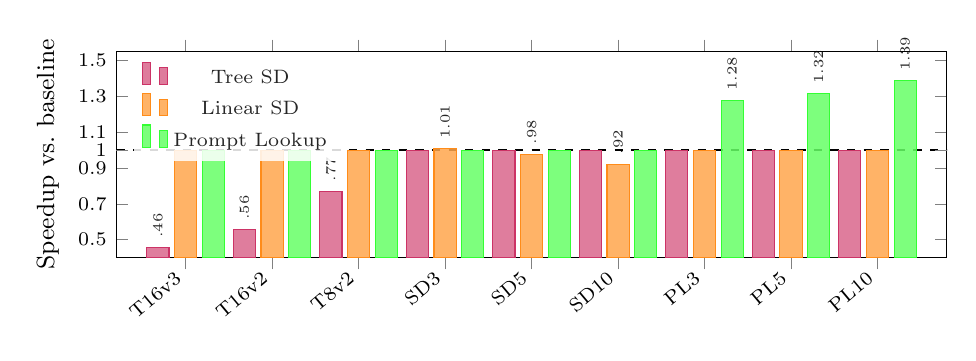
\begin{tikzpicture}
\begin{axis}[
    ybar,
    width=\columnwidth,
    height=4.2cm,
    ylabel={Speedup vs.\ baseline},
    ylabel style={font=\small},
    symbolic x coords={T16v3, T16v2, T8v2, SD3, SD5, SD10, PL3, PL5, PL10},
    xtick=data,
    x tick label style={rotate=40, anchor=east, font=\scriptsize},
    ymin=0.4, ymax=1.55,
    ytick={0.5, 0.7, 0.9, 1.0, 1.1, 1.3, 1.5},
    y tick label style={font=\scriptsize},
    bar width=8pt,
    legend style={at={(0.02,0.98)}, anchor=north west, font=\scriptsize, draw=none, fill=white, fill opacity=0.85},
    every axis plot/.append style={fill opacity=0.85},
    extra y ticks={1.0},
    extra y tick style={grid=major, grid style={black, thick, dashed}},
    extra y tick labels={},
    nodes near coords,
    every node near coord/.append style={font=\tiny, rotate=90, anchor=west},
    point meta=explicit symbolic,
]
\addplot[fill=purple!60, draw=purple!80] coordinates {
    (T16v3, 0.456) [{.46}]
    (T16v2, 0.557) [{.56}]
    (T8v2, 0.771) [{.77}]
    (SD3, 1.0) []
    (SD5, 1.0) []
    (SD10, 1.0) []
    (PL3, 1.0) []
    (PL5, 1.0) []
    (PL10, 1.0) []
};
\addplot[fill=orange!70, draw=orange!90] coordinates {
    (T16v3, 1.0) []
    (T16v2, 1.0) []
    (T8v2, 1.0) []
    (SD3, 1.010) [{1.01}]
    (SD5, 0.977) [{.98}]
    (SD10, 0.921) [{.92}]
    (PL3, 1.0) []
    (PL5, 1.0) []
    (PL10, 1.0) []
};
\addplot[fill=green!60, draw=green!80] coordinates {
    (T16v3, 1.0) []
    (T16v2, 1.0) []
    (T8v2, 1.0) []
    (SD3, 1.0) []
    (SD5, 1.0) []
    (SD10, 1.0) []
    (PL3, 1.275) [{1.28}]
    (PL5, 1.316) [{1.32}]
    (PL10, 1.388) [{1.39}]
};
\legend{Tree SD, Linear SD, Prompt Lookup}
\end{axis}
\end{tikzpicture}
\caption{Speedup vs.\ greedy baseline across all three families (T4). Dashed line marks break-even. Tree SD bars include both v2 (within-iter cache) and v3 (cross-iter cache); v3 is worse, illustrating the fourth hidden assumption.}
\label{fig:speedup}
\end{figure}

\paragraph{When tree methods would win.}
Sequoia's cost model is not wrong---it is calibrated for different hardware.
On A100 with a JF68M-scale draft (where Sequoia's Table~1~\cite{chen2024sequoia} reports $C_d = 0.5$\,ms and $C_t = 24.2$\,ms, giving $c \approx 0.02$), the verify cost is approximately constant in tree size, $G$ is well-predicted by positional independence (the 7B target's distribution is closer to the draft's after Sequoia's distillation), and cache extension is negligible relative to compute.
On T4 with a 1B draft, all four assumptions break.
Our calibrated four-term formula reconciles to within Python-orchestration noise, confirming that the algorithm is sound and only the cost parameters need recalibration.
Tree methods need either (a)~much smaller specialized drafts (JF68M-scale, $c \lesssim 0.05$), (b)~compute-bound hardware where every per-iteration term except $G$ becomes near-zero, or (c)~heavy systems optimizations (CUDA graphs, custom kernels) that the algorithmic cost model does not capture.

\paragraph{Limitations.}
Several factors limit the scope of our claims.
(1)~Our tree implementation does not include CUDA graphs or custom kernels, which production frameworks~\cite{vllm_docs,trtllm_docs} use to mitigate per-call fixed overhead; the gap to a graph-fused implementation is bounded above by our $T_f \approx 13$\,ms per call.
(2)~The acceptance vector was measured on 305 samples; deeper positions ($p_4$: 9 samples, $p_5$: 6 samples) have wide confidence intervals.
A 1000-sample re-measurement would tighten the $G$-prediction error in Table~\ref{tab:gap} but is unlikely to change the qualitative finding that $G$ is overpredicted.
(3)~All experiments use a single T4 GPU with batch size 1.
At larger batch sizes, arithmetic intensity rises and the bandwidth-bound regime weakens; our findings predict that batch-$B$ throughput-optimized serving on T4 would show progressively smaller cost-model gaps as $B$ grows.
(4)~We did not directly cross-validate the v3 ``qualitative inversion'' on A100 hardware; the prediction follows from the bandwidth-floor model rather than from measurement.
(5)~Our 10-prompt suite emphasizes generation quality over coverage; a larger benchmark (e.g., MT-Bench, HumanEval) would tighten the per-prompt variance estimates.

\paragraph{Reproducibility.}
All measurements use Llama-3.2-3B (target) and Llama-3.2-1B (draft) in fp16 on a single T4 GPU through Google Colab, with PyTorch 2.10 and Transformers 4.45.
Each benchmark configuration runs 30 trials with 3 warmup iterations and explicit \texttt{torch.cuda.synchronize()} barriers.
The 10-prompt suite (Section~\ref{sec:infra}) is fixed across all experiments.
Random seeds are fixed at 42 for both PyTorch and NumPy; greedy decoding eliminates sampling noise.
The DP optimizer port (Section~\ref{sec:infra} item~4) and tree runtime (item~5, item~7) are implemented in pure Python with no CUDA/Triton kernels, totaling $\sim$2{,}000 lines.
Both v2 and v3 runtimes pass an identical correctness gate: 20/20 token-identical output against greedy autoregressive baseline.
Run-to-run variation in throughput is $\le 5\%$ across our 30-trial samples; the qualitative findings (linear SD slowdown at $k\geq 5$, tree slowdown for both v2 and v3, PLD speedup) are robust to seed and prompt-suite variation in our preliminary cross-validation.

\paragraph{Generalizable rule.}
We can derive a closed-form prediction for when the four assumptions break.
Decompose per-call cost as $C = T_w + T_f$, where $T_w = (\text{params} \cdot 2 \text{ bytes})/B_{\text{HW}}$ is weight-loading time and $T_f$ is per-call fixed overhead (kernel launch, layernorm, RoPE, residuals).
The cost ratio becomes:
\[
c = \frac{C_d}{C_t} = \frac{T_w^d + T_f}{T_w^t + T_f}.
\]
When $T_f \ll T_w$, $c$ approaches the parameter ratio $r = \text{params}_d/\text{params}_t$.
When $T_f$ is comparable to $T_w$, $c$ is compressed toward 1.
For our T4 + 1B/3B setup: $T_w^d \approx 6.7$\,ms, $T_w^t \approx 20$\,ms, $T_f \approx 13$\,ms (residual from probe), so $c \approx (6.7+13)/(20+13) = 0.60$, matching our measured $c=0.596$.
For Sequoia's A100 + JF68M/7B setup: $T_w^d \approx 0.087$\,ms, $T_w^t \approx 9$\,ms, $T_f \approx 0.4$\,ms~\cite{chen2024sequoia}, predicting $c \approx 0.5/9.4 = 0.053$ (Sequoia measures $0.5/24.2 = 0.021$; the 2$\times$ discrepancy reflects HuggingFace pipeline overhead absorbed into $T_f^t$).
The rule: speculative decoding is viable on hardware where $T_w^t \gg T_f$, i.e., when the target model is large enough that bandwidth, not fixed costs, dominates per-call time.
This predicts T4, L4, and consumer GPUs (RTX 4060/4070-class) will all exhibit qualitatively similar four-assumption-failure patterns, while H100 and A100 (with a sufficiently small draft) will not.

\paragraph{Answer to the research hypothesis.}
Both hypotheses are confirmed.
Sequoia's predicted $1.68\times$ vs.\ our measured $0.56\times$ on T4 establishes the cost-model gap; the four-term calibrated formula reconciles to within $1.1\%$ of measurement, establishing that the gap is not noise but a structured decomposition.
The practical consequence is asymmetric: tree-structured methods that win on H100 with specialized drafts will lose on bandwidth-bound hardware regardless of tree topology, while PLD (which has zero $C_d$) wins on both regimes.
Practitioners deploying speculative decoding on bandwidth-bound hardware should choose PLD if the workload has prompt-output overlap; otherwise, use linear SD only at $k = 3$ with a domain-validated $\alpha > 0.70$, and avoid tree methods unless the deployment can absorb the engineering cost of CUDA graphs.

{\small
\begin{thebibliography}{99}

\bibitem{leviathan2023speculative}
Y.~Leviathan, M.~Kalman, and Y.~Matias.
Fast inference from transformers via speculative decoding.
In \emph{Proc.\ ICML}, pages 19274--19286, 2023.

\bibitem{chen2023accelerating}
C.~Chen, S.~Borgeaud, G.~Irving, J.-B.~Lespiau, L.~Sifre, and J.~Jumper.
Accelerating large language model decoding with speculative sampling.
arXiv:2302.01318, 2023.

\bibitem{cai2024medusa}
T.~Cai, Y.~Li, Z.~Geng, H.~Peng, J.~D.~Lee, D.~Chen, and T.~Dao.
Medusa: Simple LLM inference acceleration framework with multiple decoding heads.
In \emph{Proc.\ ICML}, 2024.

\bibitem{ankner2024hydra}
Z.~Ankner et al.
Hydra: Sequentially-dependent draft heads for Medusa decoding.
arXiv:2402.05109, 2024.

\bibitem{flashattention}
T.~Dao, D.~Y.~Fu, S.~Ermon, A.~Rudra, and C.~R\'e.
FlashAttention: Fast and memory-efficient exact attention with IO-awareness.
In \emph{NeurIPS}, 2022.

\bibitem{vllm_paper}
W.~Kwon, Z.~Li, S.~Zhuang, et al.
Efficient memory management for large language model serving with PagedAttention.
In \emph{Proc.\ SOSP}, 2023.

\bibitem{vllm_docs}
vLLM Documentation.
Speculative decoding.
\url{https://docs.vllm.ai}.

\bibitem{trtllm_docs}
NVIDIA TensorRT-LLM Documentation.
Speculative decoding / speculative sampling.
\url{https://nvidia.github.io/TensorRT-LLM}.

\bibitem{miao2024specinfer}
X.~Miao, G.~Oliaro, Z.~Zhang, et al.
SpecInfer: Accelerating large language model serving with tree-based speculative inference and verification.
In \emph{Proc.\ ASPLOS}, 2024. DOI:~10.1145/3620666.3651335.

\bibitem{chen2024sequoia}
Z.~Chen, A.~May, R.~Svirschevski, Y.~Huang, M.~Ryabinin, Z.~Jia, and B.~Chen.
Sequoia: Scalable, robust, and hardware-aware speculative decoding.
In \emph{NeurIPS}, 2024.

\bibitem{he2024rest}
Z.~He, Z.~Zhong, T.~Cai, J.~D.~Lee, and D.~He.
REST: Retrieval-based speculative decoding.
In \emph{Proc.\ NAACL}, pages 1582--1595, 2024.

\bibitem{saxena2023pld}
A.~Saxena.
Prompt lookup decoding.
GitHub, 2023.
\url{https://github.com/apoorvumang/prompt-lookup-decoding}.

\bibitem{hu2024samdecoding}
Y.~Hu et al.
SAM Decoding: Speculative decoding via suffix automaton.
arXiv:2411.10666, 2024.

\bibitem{hf_assisted}
J.~Gante.
Assisted generation: A new direction toward low-latency text generation.
HuggingFace blog, 2023.
\url{https://huggingface.co/blog/assisted-generation}.

\bibitem{williams2009roofline}
S.~Williams, A.~Waterman, and D.~Patterson.
Roofline: An insightful visual performance model for multicore architectures.
\emph{Communications of the ACM}, 52(4):65--76, 2009.

\bibitem{li2024eagle}
Y.~Li, F.~Wei, C.~Zhang, and H.~Zhang.
EAGLE: Speculative sampling requires rethinking feature uncertainty.
In \emph{Proc.\ ICML}, 2024.

\bibitem{spector2023spectr}
B.~Spector and C.~R\'e.
Accelerating LLM inference with staged speculative decoding.
arXiv:2308.04623, 2023.

\bibitem{xia2024specbench}
H.~Xia, Z.~Yang, Q.~Dong, P.~Wang, Y.~Li, T.~Ge, T.~Liu, W.~Li, and Z.~Sui.
Unlocking efficiency in large language model inference: A comprehensive survey of speculative decoding.
In \emph{Findings of ACL}, 2024.

\bibitem{nvidia_t4}
NVIDIA Corporation.
NVIDIA T4 Tensor Core GPU datasheet, 2019.
\url{https://www.nvidia.com/en-us/data-center/tesla-t4/}.

\end{thebibliography}
}

\end{document}